\chapter{Results}
\label{chap:results}
In this chapter the results of the classification using “Max MCC” optimization strategy are presented. Some premises are necessary before proceeding with the interpretation of the data:
\begin{enumerate}
\item 	The average scores at the bottom of each table are between models with the same architecture, but different hyper-parameters. Furthermore, as part of the "Max MCC" strategy, having an accuracy lower than the majority class guessing (defined as "chance level" in the tables) but with a positive \ac{MCC} has been preferred compared to having the highest possible accuracy with a zero or negative \ac{MCC}.
\item 	All models are underfitting or overfitting to some degree on their dataset but, considering the challenges of classifying emotions, models with positive \ac{MCC} and \ac{CV MCC} are reported as good models regardless their scoring. As a consequence, only extreme cases of overfitting, i.e. models with 0 or negative \ac{MCC} and positive \ac{CV MCC}, and extreme case of underfitting, i.e. models with 0 or negative \ac{CV MCC} are labelled as such in tables \ref{tbl:arousal_results} and \ref{tbl:valence_results}.
\item 	CV Accuracy, CV Acc Std, \ac{CV MCC} and CV MCC Std stand for Cross-Validated Accuracy and MCC and their respective standard deviation.
\item 	Test accuracy and \ac{MCC} are computed using an unseen test split of the data. CV Accuracy and \ac{CV MCC} have been computed on the training split of the data; thus, their purpose is to provide a measure of consistency of the test scores (see Fig \ref{fig_data_split_strategy}).
\item 	The confidence interval has been calculated on the test split, Z=1.96. 
\item 	Chance level represents the default guessing of the majority class.
\item 	Standard deviation of each measure, if present, is between round parenthesis in the tables.
\end{enumerate}

First, the classification performances of \ac{SVM} and \ac{MLP} are compared for both arousal and valence classification. Then, the results are compared with related work.

\section{Support-Vector Machines vs Multi-Layer Perceptron}
\label{sec:svm_mlp}
The results of the subject-dependent arousal classification experiment are reported in Table \ref{tbl:arousal_results}, while the results for valence classification are reported in Table \ref{tbl:valence_results}. In these tables, learning models can be identified by a positive \ac{MCC} score supported by a positive \ac{CV MCC} and are highlighted in blue. The models that over-fitted, highlighted in yellow, are characterized by negative \ac{MCC} and positive \ac{CV MCC}, meaning that they learned well on the training data but could not discriminate classes on the test data. Under-fitted models instead are characterized by zero or negative \ac{CV MCC} and positive or negative \ac{MCC}, because they did not have the adequate capabilities to capture the underlying structure of the training data, but possibly obtained a good test accuracy by random guessing and they are highlighted in orange.  In arousal classification the average majority class guessing (defined as chance level in the table) is \(58\pm8\%\), the highest and consistent test accuracy score is \(84\%\) with \ac{MCC} score of \(0.20\) using \ac{SVM} and \(88\%\) with \ac{MCC} score of \(0.78\) using \ac{MLP}. For \ac{SVM} classifiers, the average test accuracy is \( 61\pm9\%\) with average MCC of \(0.16\pm0.20\), \(61\pm6\% \) \ac{CV} accuracy and \ac{CV MCC} of \(0.24\pm0.12\). For \ac{MLP} classifiers, the average test accuracy is \(58\pm12\%\), with average MCC of \(0.13\pm0.20\), \(57\pm8\% \) \ac{CV} accuracy and \ac{CV MCC} of \(0.15\pm0.16\). 

\begin{table}[h!]
  \caption{Arousal classification results using MCC as scoring parameter for GridSearch. Learning models are highlighted in blue, over-fitted and under-fitted models are highlighted in yellow and orange, respectively.}
  \label{tbl:arousal_results}
  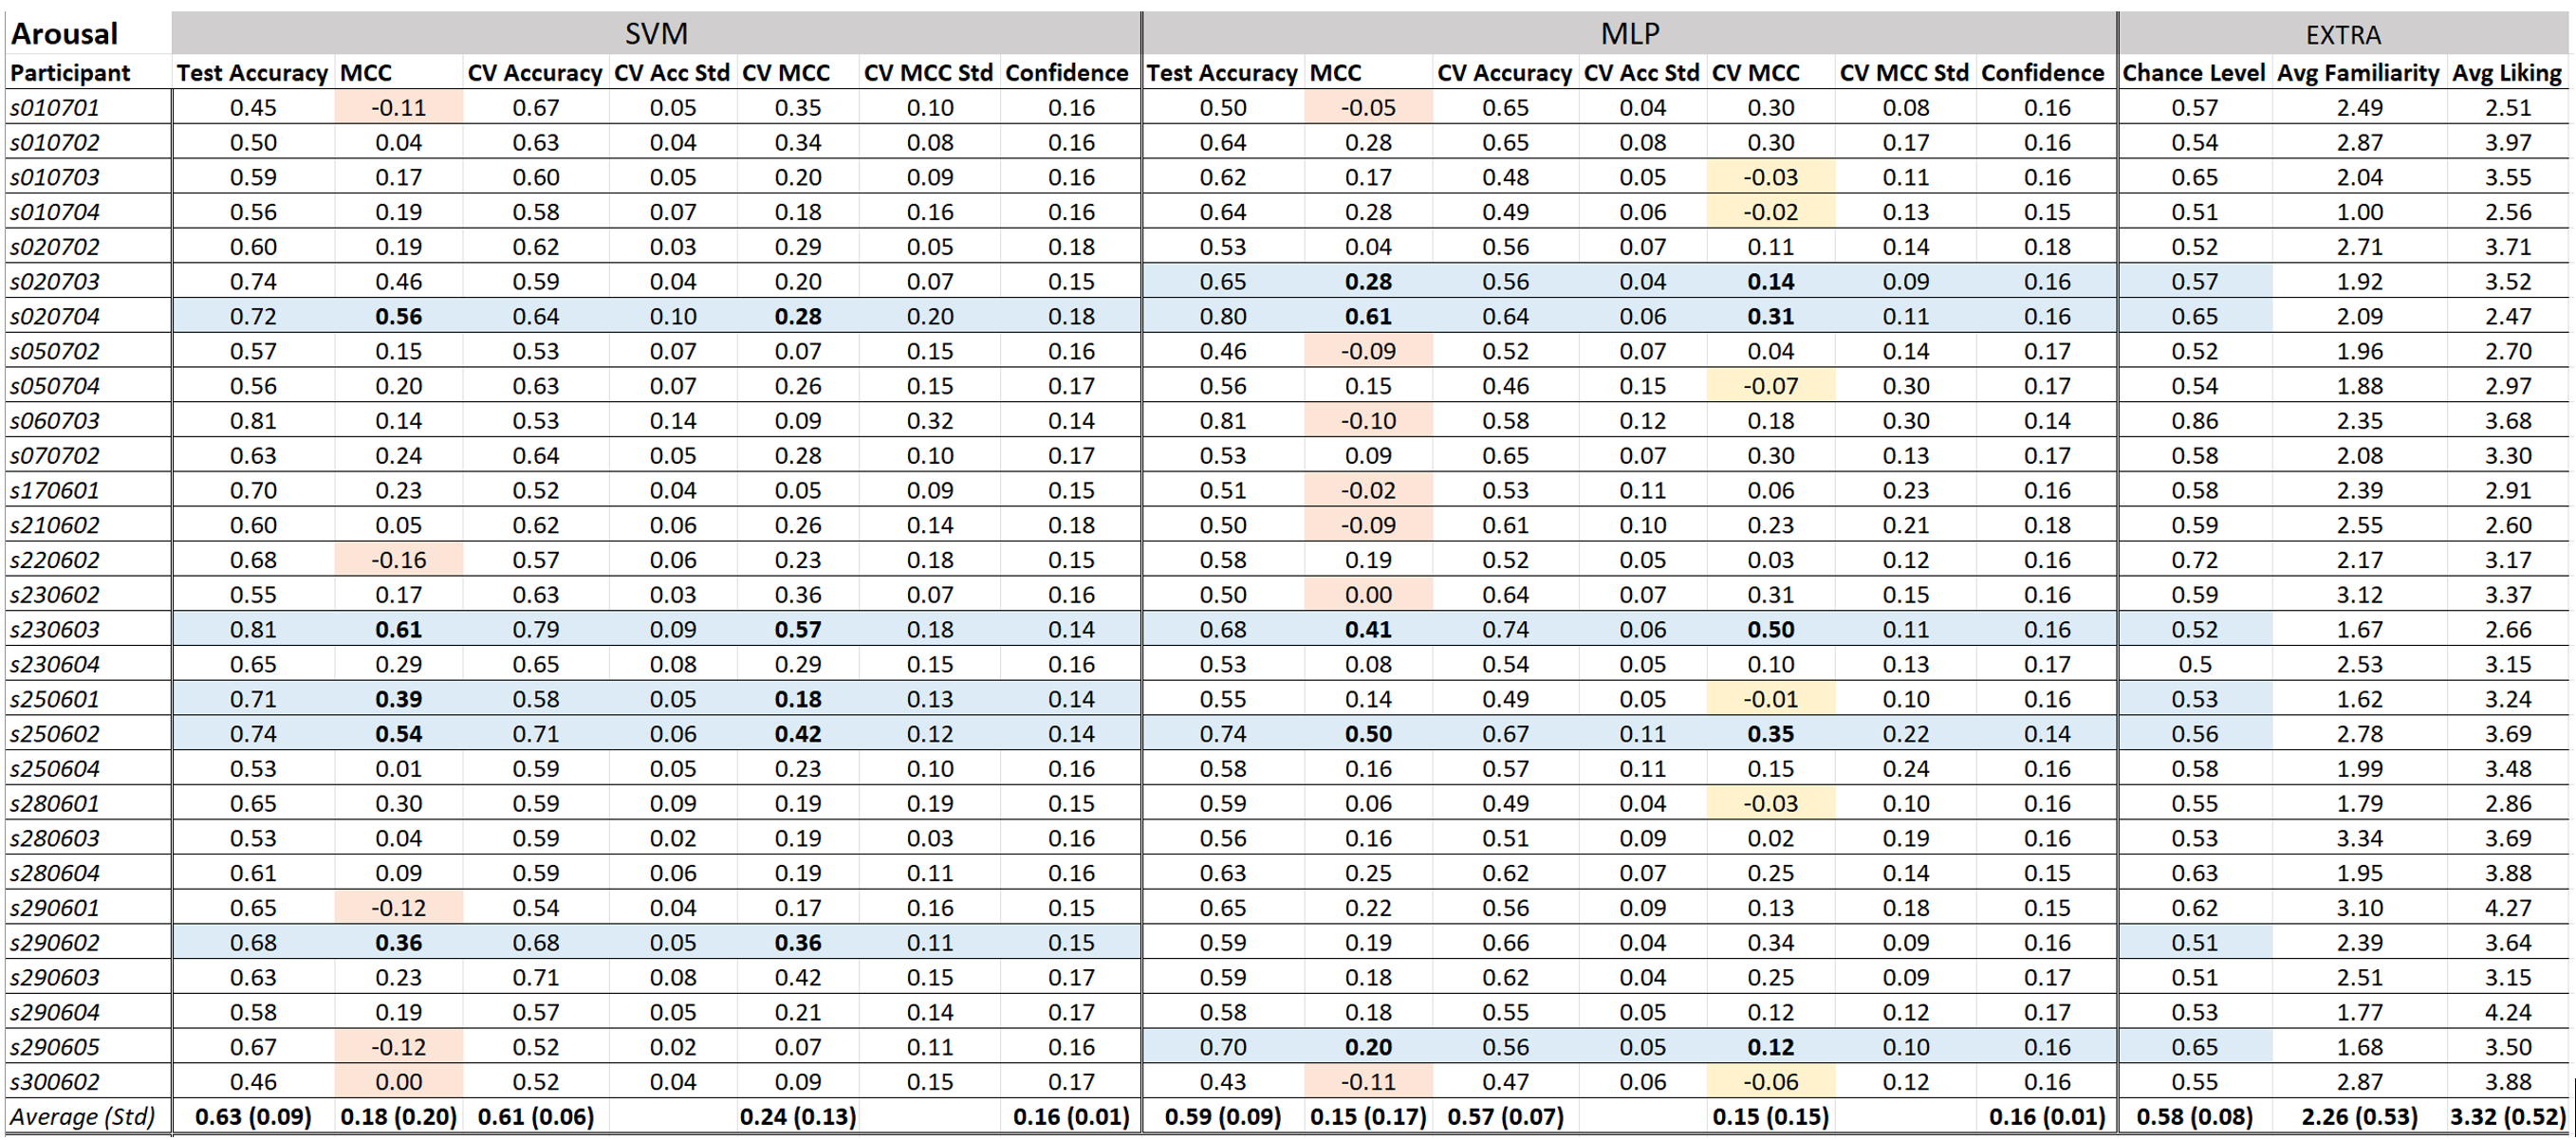
\includegraphics[width=\linewidth]{img/results/arousal_results.png}
\end{table}

In valence classification (see Table \ref{tbl:valence_results}) the average majority class guessing (defined as chance level in the table) is \(65\pm12\%\), the highest and consistent test accuracy score is \(89\%\) with \ac{MCC} score of \(0.27\) using \ac{SVM} and \(77\%\) with \ac{MCC} score of \(0.48\) using \ac{MLP}. For \ac{SVM} classifiers, the average test accuracy is \( 67\pm12\%\) with average MCC of \(0.13\pm0.18\), \(61\pm6\% \) \ac{CV} accuracy and \ac{CV MCC} of \(0.26\pm0.13\). For \ac{MLP} classifiers, the average test accuracy is \(65\pm12\%\), with average MCC of \(0.11\pm0.18\), \(56\pm9\% \) \ac{CV} accuracy and \ac{CV MCC} of \(0.13\pm0.18\). The large variances are affected by the unbalanced distribution of positive and negative classes (see Chapter \ref{sec:unbalanced_labelling}), but it are also a clear symptom of diffused over-fitting, especially for \ac{MLP} classifiers. 

\begin{table}[h!]
  \caption{Valence classification results using MCC as scoring parameter for GridSearch. Learning models are highlighted in blue, over-fitted and under-fitted models are highlighted in yellow and orange, respectively.}
  \label{tbl:valence_results}
  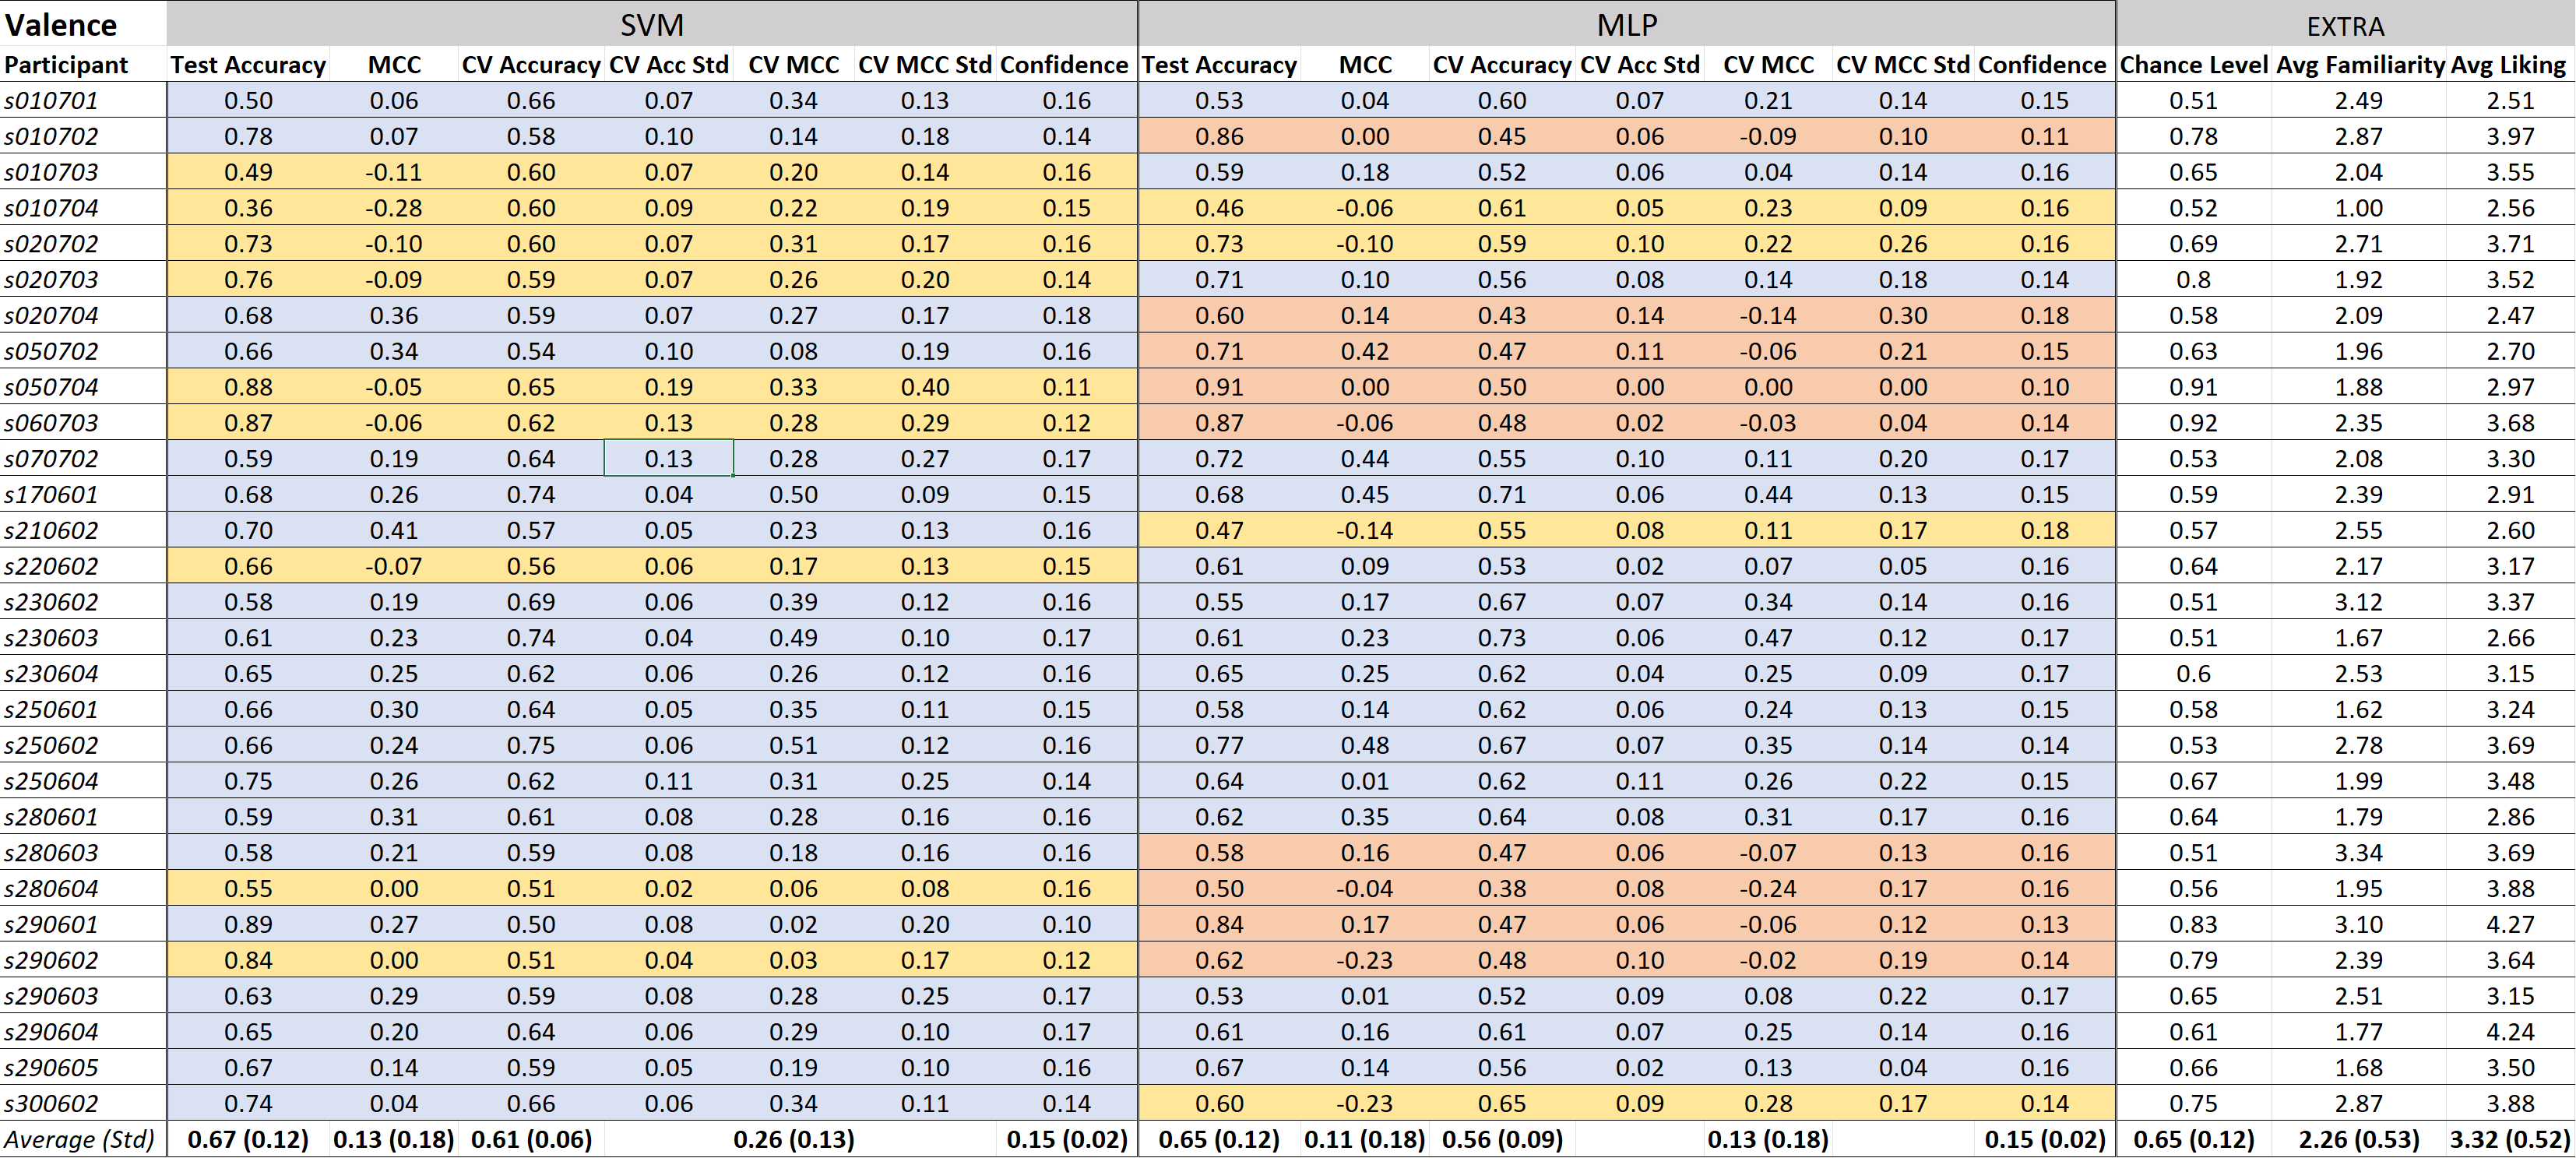
\includegraphics[width=\linewidth]{img/results/valence_results.png}
\end{table}

A final remark can be obtained by comparing the number of learning, over-fitting and under-fitting models between the two type of classifiers (see Fig. \ref{fig:svm_vs_mlp}. In arousal classification it was possible to train 25 \ac{SVM} learning classifiers, with 4 over-fitting models and 0 under-fitting models against 15 \ac{MLP} learning classifiers, 6 over-fitting models and 8 under-fitting models. In valence classification it was possible to train 20 \ac{SVM} learning classifiers, with 9 over-fitting models and 0 under-fitting models against 17 \ac{MLP} learning classifiers, 4 over-fitting models and 8 under-fitting models. 
Overall, the classification performances between \ac{SVM} and \ac{MLP} are not significantly different, but \ac{SVM} proved to be more reliable and obtained average classification accuracy above the majority default guessing threshold and generated more models able to discriminate unseen data. The are other model-specific advantages and disadvantages a to be taken into account in the implementation of a real-time application, for example most \ac{MLP} implementations support partial fitting of the models that is very useful with continuous streams of data, however these technical considerations lie outside the scope of this research.

\begin{figure}[h!]
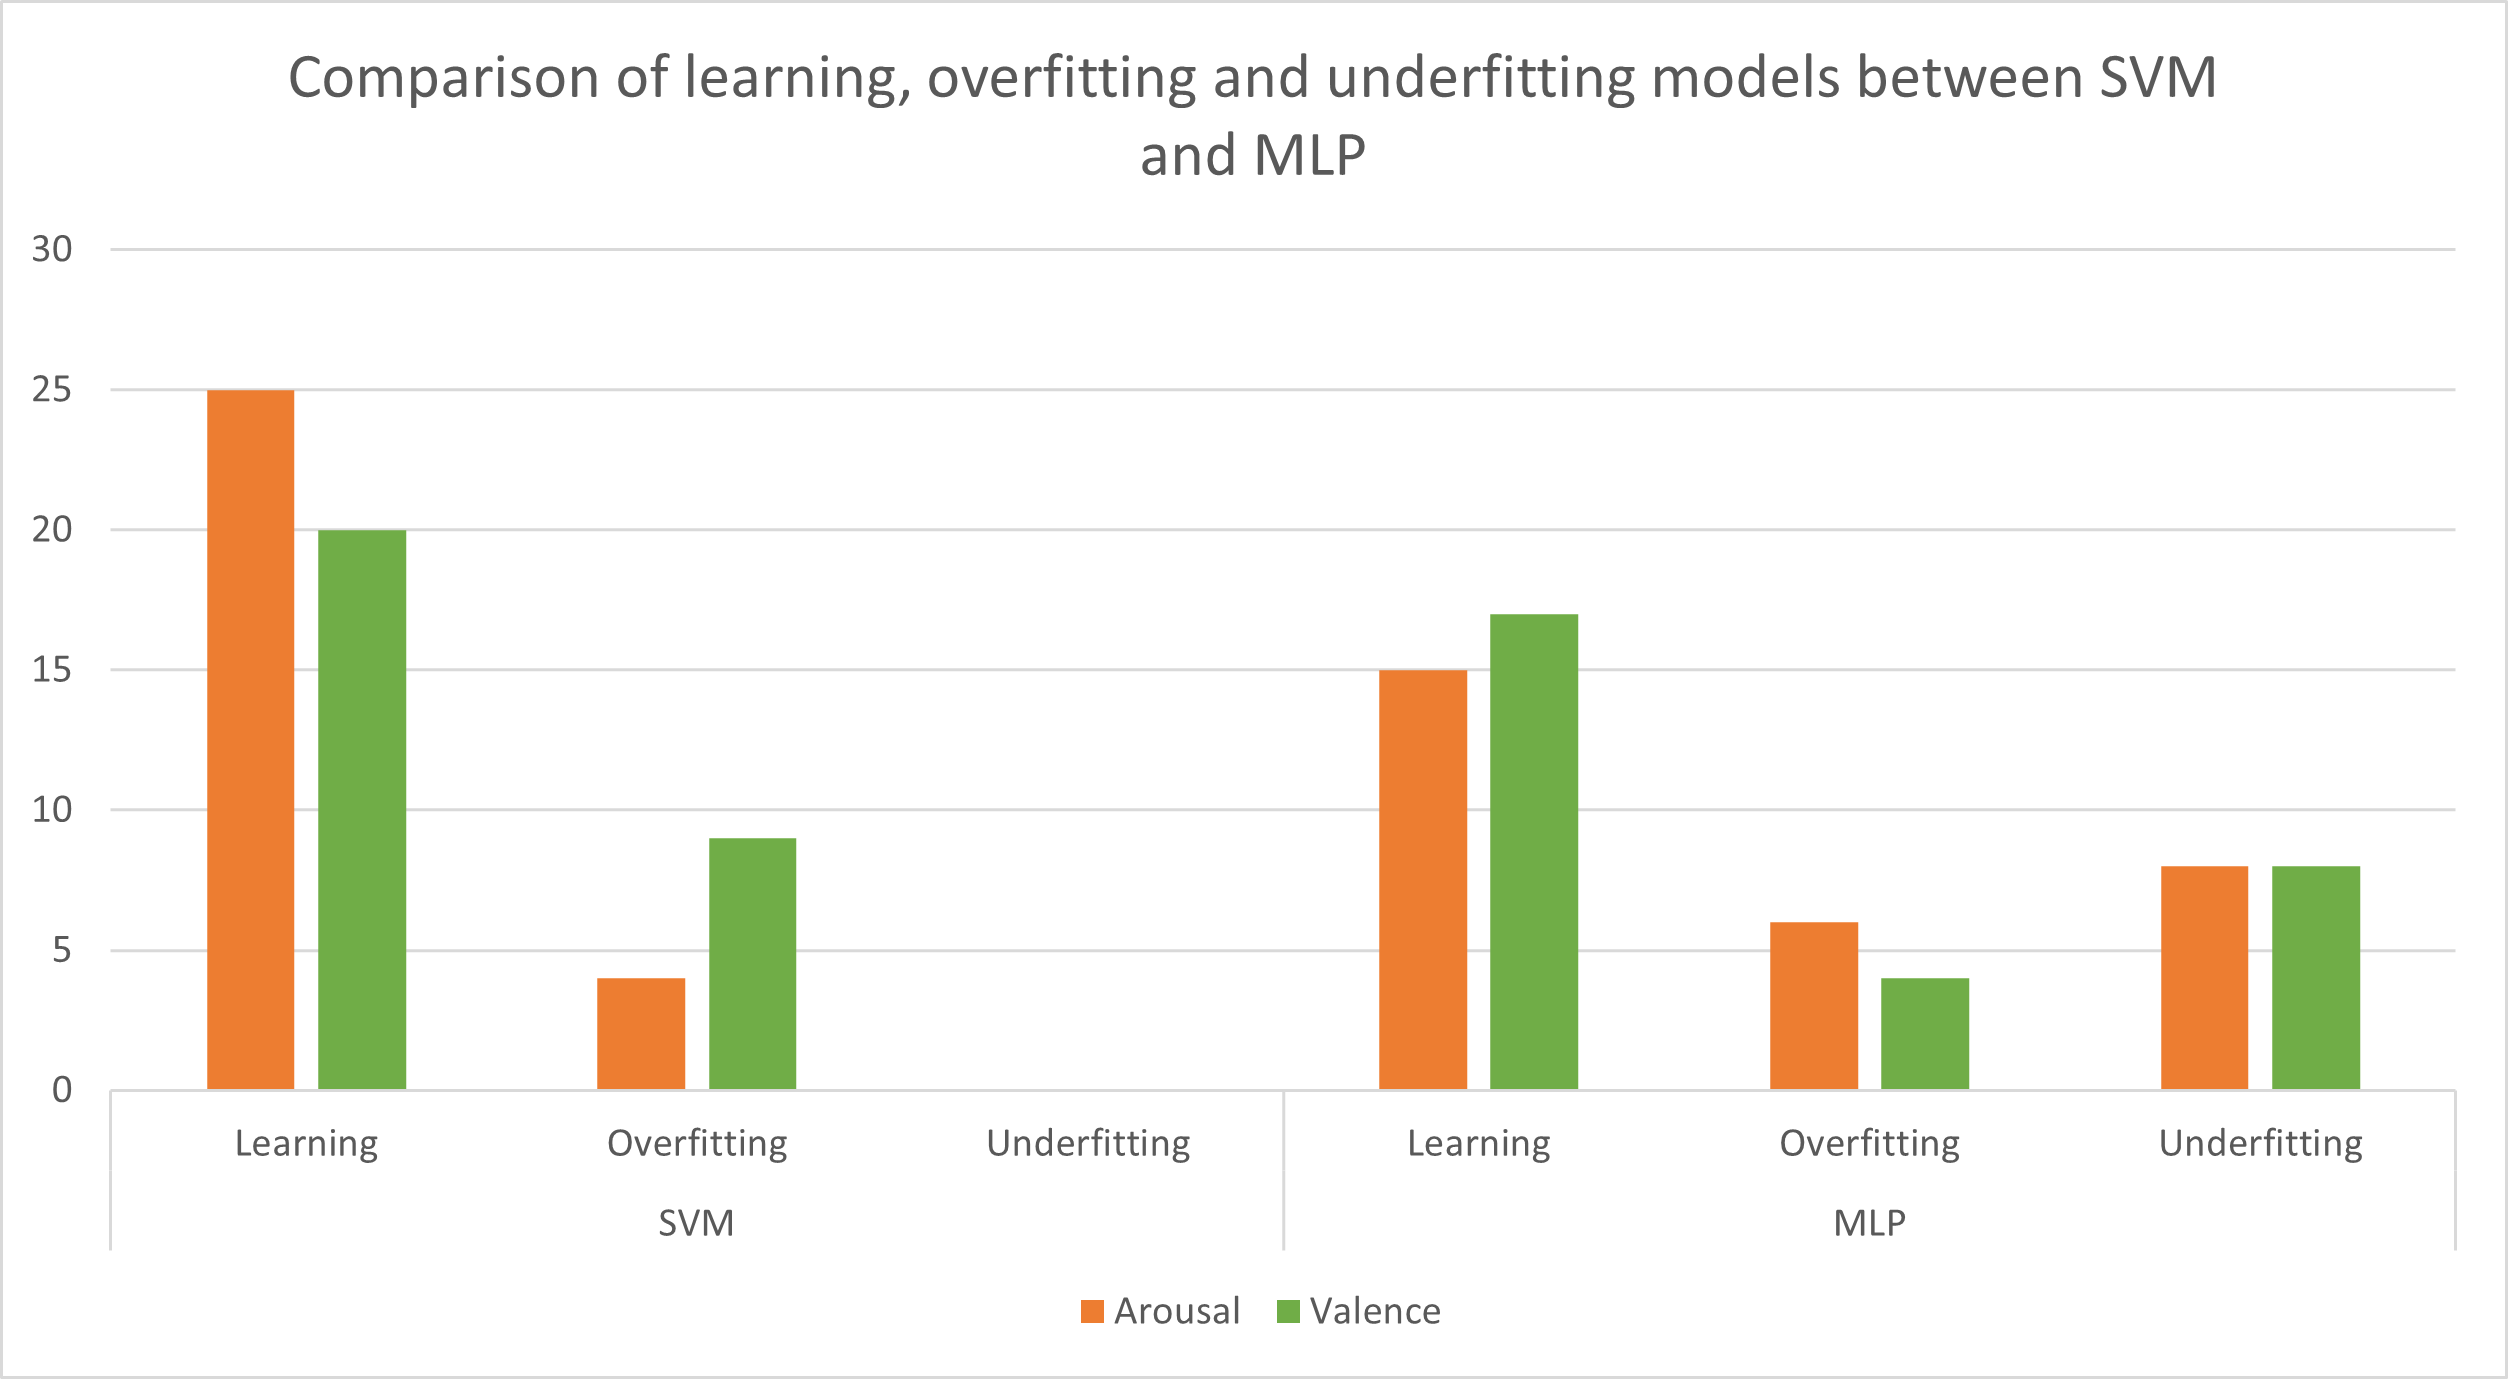
\includegraphics[width=12cm]{img/results/svm_vs_mlp.png}
\centering
\caption{Comparison of SVM and MLP in terms of number of learning, overfitting and underfitting models.} \label{fig:svm_vs_mlp}
\end{figure}



\section{Comparison with related work}
\label{sec:comparison}
Comparing the result of the current research with related work is non-trivial because of the methodological differences in data collection, processing, and evaluation. These differences have been considered to sort the comparisons from most comparable to least comparable. 
\\
The first and most comparable study \cite{thammasan_multimodal_2017} used self-reported continuous annotation as main labelling method for classification, the data were collected from 9 subjects with a wearable EEG headset equipped with 8 dry electrodes and processed using the automated PREP pipeline in MATLAB. The accuracy scores of \ac{SVM} classifiers using EEG and \ac{LOBO} cross-validation are only reported through plots, valence classification scored average accuracy of ~\(68\pm10\%\) and arousal classification scored average accuracy ~\(64\pm10\%\) . The comparison only takes into account results from \ac{SVM} classifiers, which in the current study reports average test accuracy of \( 67\pm12\%\) and average LOBO cross-validated accuracy on the training set of \(61\pm6\% \)  for valence classification . Arousal classification scored an average test accuracy of  \( 61\pm9\%\) and average \ac{LOBO} cross-validated accuracy of \(61\pm6\% \). They provided a table reporting the \ac{MCC} scores for each classification modality, the average CV MCC reported for valence is \(0.247\pm0.17\) and the average \ac{CV MCC} for arousal is \(0.177\pm0.04\). The current study reports average test \ac{MCC} score of \(0.13\pm0.18\) and average \ac{CV MCC} score of \(0.26\pm0.13\) for valence, while for arousal the average test \ac{MCC} score is \(0.16\pm0.20\) and average CV MCC score is \(0.24\pm0.12\). Finally, the highest \ac{CV MCC} score reported for a single subject is \(0.596\pm0.30\) for valence and \(0.23\pm0.22\) for arousal, while in the current study the highest \ac{CV MCC} score reported is \(0.51\pm0.12\) for valence and \(0.57\pm0.18\) for arousal. These results are aligned with the current study and provide individual insights for each subject that can be easily compared, so in conclusion if we consider only the single EEG modality from \cite{thammasan_multimodal_2017}, the learning capabilities of the models trained in the current study are similar despite a lighter pre-processing and a lower number of electrodes. This comparison suggests that there definitely is room for improving the software pipeline on the current dataset, especially the \ac{AuPP}, to generate more stable models with lower variance and risk of over-fitting and under-fitting even before considering an improvement of the hardware equipment and another data collection phase.
\\
The second comparable study \cite{thammasan_continuous_2016} is the one that inspired the self-reporting of emotions using continuous annotation. The focus of this study, however, was to compare traditional discrete annotations to continuous annotation and to evaluate two approaches for features extraction. For comparison purposes, the scores reported using\ac{PSD} features will be considered instead of the scores obtained with \ac{FD} features. The accuracy scores, and relative standard deviations are mostly reported in plots and partially during the discussion, so an estimate is provided. Using \ac{SVM}, valence classification score is ~\(81.2\pm8\% \) average \ac{CV} accuracy and arousal classification score is ~\(75\pm8\%\) average CV accuracy. With MLP, valence classification score is ~\(80.2\pm10\%\) average \ac{CV} accuracy and arousal classification score is ~\(75\pm10\% \) average \ac{CV} accuracy. These scores are significantly higher than default guessing of the majority class and clearly outperform the results obtained in the current study, that are not on average significantly different than default guessing. No further insights are provided on subject-dependent performances, nor on \ac{MCC} scores, but their models are consistently reliable in performing better than default guessing. This comparison suggest that the choice of stimuli, i.e. music with or without lyrics and the distribution of emotional classes, can highly impact on the classification performances. Furthermore, improving the features engineering part to take full advantage of the continuous annotations, for example applying a sliding window segmentation technique on the \ac{EEG} data, can help better capturing the underlying emotional fluctuation. Finally, they also dealt more aggressively on unbalanced datasets, for example by removing those subjects where one of the two binary classes (either in arousal or valence classification) was missing.
\\ \
The third study \cite{wu_estimation_2017} aimed at artificially simulating a wearable device by selecting, 2, 4 and then 8 frontal electrodes from the subjects of the DEAP \cite{koelstra_deap_2012} dataset, collected with and EEG system with 32 wet electrodes and discrete self-reported labels. The asymmetry indexes used in this study are sim Only the results for the 2 electrodes configuration using \ac{SVM} for subject-dependent classification are reported and no specific description of the preprocessing pipeline is provided, so the assumption is that they used the data already preprocessed by the original authors of the dataset. The average \ac{CV} accuracy scored for valence classification is ~\(68.4\pm2.0\%\). The authors also present better accuracy scores using \ac{GBDT} and Random Forests classifiers, achieving respectively \(75.10\pm2\%\) and \(72.15\pm2\%\) accuracy for subject-dependent classification, and subsequently reported \(61.82\% \)accuracy for subject-independent classification using \ac{GBDT}. A balancing strategy for the labels is explained, but no specific distribution of positive and negative class is provided, nor individual insights for subject-dependent classification so it is not possible to evaluate the reliability of the accuracy scores compared to default guessing the majority class. In conclusion, even assuming an equal distribution of positive and negative labels, this study results with \ac{SVM} are in line with the \( 67\pm12\%\) average test accuracy in valence classification of the current research, but with a definitely lower average variance that suggests that models trained were less prone to over-fitting. In addition, this comparison suggest that other supervised learning algorithms that are constituted by ensembles of weaker classifiers, for example Random Forests and \ac{GBDT} (that is conceptually similar), can obtain much better performances than simpler models such as \ac{SVM} and \ac{MLP}.
\\
The fourth and last comparable study \cite{lin_eeg-based_2009} collected self-reported continuous annotations from 26 subjects using a standard EEG system with 32 wet electrodes. The data were preprocessed with visual inspection on EEGLab and then features were extracted from 12 pairs of symmetrical electrodes. The authors provide 3 classifications schemes, but only the “one-against-one scheme is comparable in terms of binary classification of valence and arousal and therefore reported. The reported average \ac{CV} accuracy score for valence classification is \(94.86\pm17.6\%\)  and for arousal classification is \(94.43\pm21.2\%\). The authors did not report the distribution of the classes for each subject so it is not possible to evaluate the reliability of the accuracy scores for each subject. The high average variance suggests that they also generated a number of over-fitted models, similarly to the current study, nevertheless their follow-up study \cite{lin_eeg-based_2010} applied a better features engineering process that lowered the overall variance that enabled them to obtain a lower but more stable average classification accuracy of \(82.29\pm3.06\% \) of four emotional states (joy, anger, sadness and pleasure) using \ac{SVM} and even to identify 30 subject-independent features relevant to emotional processing across subjects. These studies by Lin et al. report interesting strategies for selecting and ranking EEG features for the transition from subject-dependent classification to subject-independent classification, however after experimenting with electrodes reduction their models performances dramatically dropped when the electrodes number was lower than 18 (9 pairs), suggesting that subject-independent classification is still out of reach of wearable devices like Melomind.
